\usetikzlibrary{arrows.meta, positioning, calc}

\definecolor{layerA}{HTML}{355B8C}
\definecolor{layerB}{HTML}{4A6FA5}
\definecolor{layerC}{HTML}{7C93BD}
\definecolor{arrowgray}{HTML}{888888}
\definecolor{notecolor}{HTML}{666666}

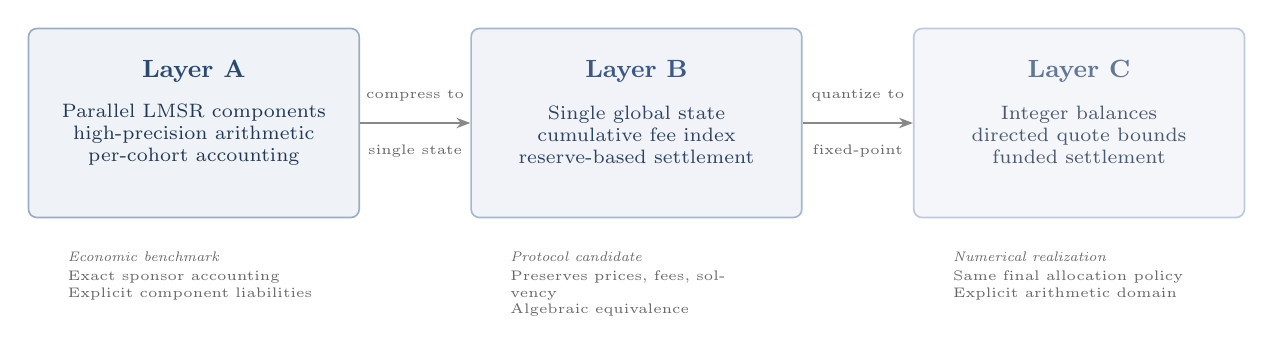
\begin{tikzpicture}[
  layer/.style={
    rectangle,
    rounded corners=3pt,
    minimum width=4.2cm,
    minimum height=2.4cm,
    draw=#1!50,
    fill=#1!8,
    line width=0.6pt,
    inner sep=0pt,
  },
  layertitle/.style={
    font=\small\bfseries,
    #1!80!black,
  },
  layerdesc/.style={
    font=\scriptsize,
    #1!60!black,
    align=center,
    text width=3.4cm,
  },
  preserves/.style={
    font=\tiny,
    notecolor,
    align=left,
    text width=3.2cm,
  },
  arrowlabel/.style={
    font=\tiny,
    notecolor,
    align=center,
  },
]

% Layer A
\node[layer=layerA] (A) {};
\node[layertitle=layerA] at ($(A.north)-(0,0.55)$) {Layer A};
\node[layerdesc=layerA] at ($(A.center)+(0,-0.15)$) {Parallel LMSR components\\high-precision arithmetic\\per-cohort accounting};

% Layer B
\node[layer=layerB, right=1.4cm of A] (B) {};
\node[layertitle=layerB] at ($(B.north)-(0,0.55)$) {Layer B};
\node[layerdesc=layerB] at ($(B.center)+(0,-0.15)$) {Single global state\\cumulative fee index\\reserve-based settlement};

% Layer C
\node[layer=layerC, right=1.4cm of B] (C) {};
\node[layertitle=layerC] at ($(C.north)-(0,0.55)$) {Layer C};
\node[layerdesc=layerC] at ($(C.center)+(0,-0.15)$) {Integer balances\\directed quote bounds\\funded settlement};

% Arrows
\draw[-{Stealth[length=5pt]}, arrowgray, thick]
  (A.east) -- (B.west)
  node[arrowlabel, midway, above=4pt] {compress to}
  node[arrowlabel, midway, below=4pt] {single state};

\draw[-{Stealth[length=5pt]}, arrowgray, thick]
  (B.east) -- (C.west)
  node[arrowlabel, midway, above=4pt] {quantize to}
  node[arrowlabel, midway, below=4pt] {fixed-point};

% Role labels below
\node[preserves=layerA, anchor=north] at ($(A.south)-(0,0.3)$) {
  \textit{Economic benchmark}\\[1pt]
  Exact sponsor accounting\\
  Explicit component liabilities
};

\node[preserves=layerB, anchor=north] at ($(B.south)-(0,0.3)$) {
  \textit{Protocol candidate}\\[1pt]
  Preserves prices, fees, solvency\\
  Algebraic equivalence
};

\node[preserves=layerC, anchor=north] at ($(C.south)-(0,0.3)$) {
  \textit{Numerical realization}\\[1pt]
  Same final allocation policy\\
  Explicit arithmetic domain
};

\end{tikzpicture}
